\section{OpenMP v5.2}

\subsection{Introduction}

\definition{OpenMP} is a scalable model that gives parallel programmers a simple and flexible interface for developing portable parallel applications in C/C++ and Fortran.
\begin{itemize}
    \item \textbf{Header file} to include in the main file: \texttt{omp.h}.
    \item To \texttt{compile} and use it, it is necessary to add the \texttt{flag} \texttt{-fopenmp} to the gcc (or c++) options.
\end{itemize}
The following link contains about 200 slides on OpenMP. It is an introduction, but it covers every argument required in this PoliMI course. The slides are made by a Senior Principal Engineer, Mattson Tim. He's a Senior Principal Engineer at Intel, where he's been since 1993. The \href{https://www.openmp.org/wp-content/uploads/Intro_To_OpenMP_Mattson.pdf}{slide link}.
\begin{flushleft}
    \textcolor{Green3}{\faIcon{check} \textbf{Benefits}}
\end{flushleft}
\begin{itemize}
    \item Standard across a variety of shared memory architectures and platforms.
    \item Supports three famous languages: Fortran, C and C++.
    \item Scalable from embedded systems to the supercomputer.
    \item The directives are intuitive, and with a limited set of directives we can implement parallel algorithms.
    \item Incremental parallelization of serial program.
    \item Coarse-grained and fine-grained parallelism. See \href{https://www.geeksforgeeks.org/difference-between-fine-grained-and-coarse-grained-simd-architecture/}{here} here an interesting difference between coarse-grained and fine-grained architecture:
    \begin{center}
        \qrcode{https://www.geeksforgeeks.org/difference-between-fine-grained-and-coarse-grained-simd-architecture/}
    \end{center}
\end{itemize}

\begin{flushleft}
    \textcolor{Green3}{\faIcon{question-circle} \textbf{How it works?}}
\end{flushleft}
OpenMP is based on the \textbf{fork-join paradigm}. A \dquotes{master} thread forks a specified number of \dquotes{slave} threads. Tasks are divided among the \dquotes{slaves}, and each \dquotes{slave} runs concurrently as the runtime allocates threads to different processors.
\begin{enumerate}
    \item \textbf{\texttt{Thread \#0} born}. OpenMP programs start with a single thread;
    \item \textbf{Fork}. At the start of a parallel region, the \emph{master} creates a team of parallel worker threads (\emph{slaves}).
    \item \textbf{OpenMP code block}. Statements in the parallel block are executed in parallel by each thread.
    \item \textbf{Join}. At the end of the parallel region, all threads synchronize (implicit barrier, see definition on page \pageref{paragraph: Joining through Barriers}) and join the master thread.\cite{whatIsOpenMPumassJohnstonHans}
\end{enumerate}

\newpage

\begin{figure}[!htp]
    \centering
    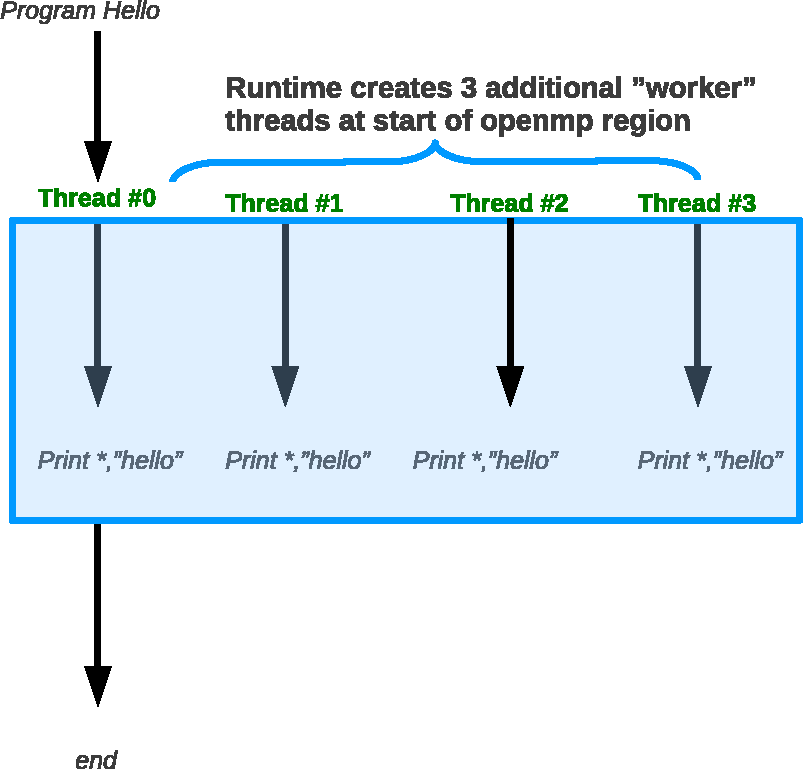
\includegraphics[width=.7\textwidth]{img/openmp-1.pdf}
    \caption{Example of an OpenMP program called \texttt{Hello}. At runtime, the \emph{master} thread forks 3 additional \emph{slave} threads to print \texttt{hello}. The example is very trivial, but here is a graphical representation of the workflow. An interesting thing to note is that \textbf{OpenMP creates} a sort of \textbf{region where each thread executes all the instructions in the OpenMP block}. This is important to understand.\cite{whatIsOpenMPumassJohnstonHans}}
    \label{figure: how OpenMP works}
\end{figure}